\documentclass[10pt,a4paper]{article}
\usepackage[margin=2.0cm]{geometry}
\usepackage[T1]{fontenc}
\usepackage{lmodern,microtype}
\usepackage{graphicx,booktabs,array,tabularx,longtable,float,caption}
\usepackage[table]{xcolor}
\usepackage{pgfplots}
\pgfplotsset{compat=1.18}
\usepackage{tikz}
\usetikzlibrary{arrows.meta,positioning}
\usepackage{csquotes}
\usepackage[colorlinks=true,citecolor=blue!55!black,linkcolor=blue!55!black,urlcolor=blue!55!black]{hyperref}
\usepackage[backend=biber,style=ieee,sorting=none,doi=true,url=false]{biblatex}
\addbibresource{references.bib}
\definecolor{teal}{RGB}{21,120,135}
\renewcommand{\arraystretch}{1.16}
\setlength{\parskip}{4pt}
\emergencystretch=3em
\title{Microplastic Pollution in Freshwater\\\large Four-Subtopic Literature Map and Method--Effect Evidence Tables}
\author{Y3 Group Project\\vesh sivi}
\date{October 2026}
\begin{document}
\maketitle
\begin{abstract}
This draft summarises four overlapping sets derived from 10,833 preliminary Web of Science--Scopus include candidates: Causes (6,430), Water Effects (7,575), Laboratory Methods (6,654) and Data Trends (5,320). Tables and PGFPlots charts list every \emph{defined} subcategory and its automated title/abstract match frequency. A second table under each theme gives examples of methods and abstract-reported findings with indexed IEEE citations. The review supports planning a reference-laboratory validation strategy; it is \textbf{not a final full-text systematic review}. Subcategory frequencies are multi-label and must not be interpreted as experimentally established effects.
\end{abstract}
\section{Literature identification and classification}
From 18,942 database records (8,923 Web of Science; 10,019 Scopus), deduplication removed 7,318 records and document-type filtering excluded 727. The remaining 10,897 records yielded 10,833 preliminary include candidates and 64 requiring manual review. Four overlapping top-level themes were assigned to candidate papers; these are not four mutually exclusive bodies of evidence.
\begin{figure}[H]
\centering
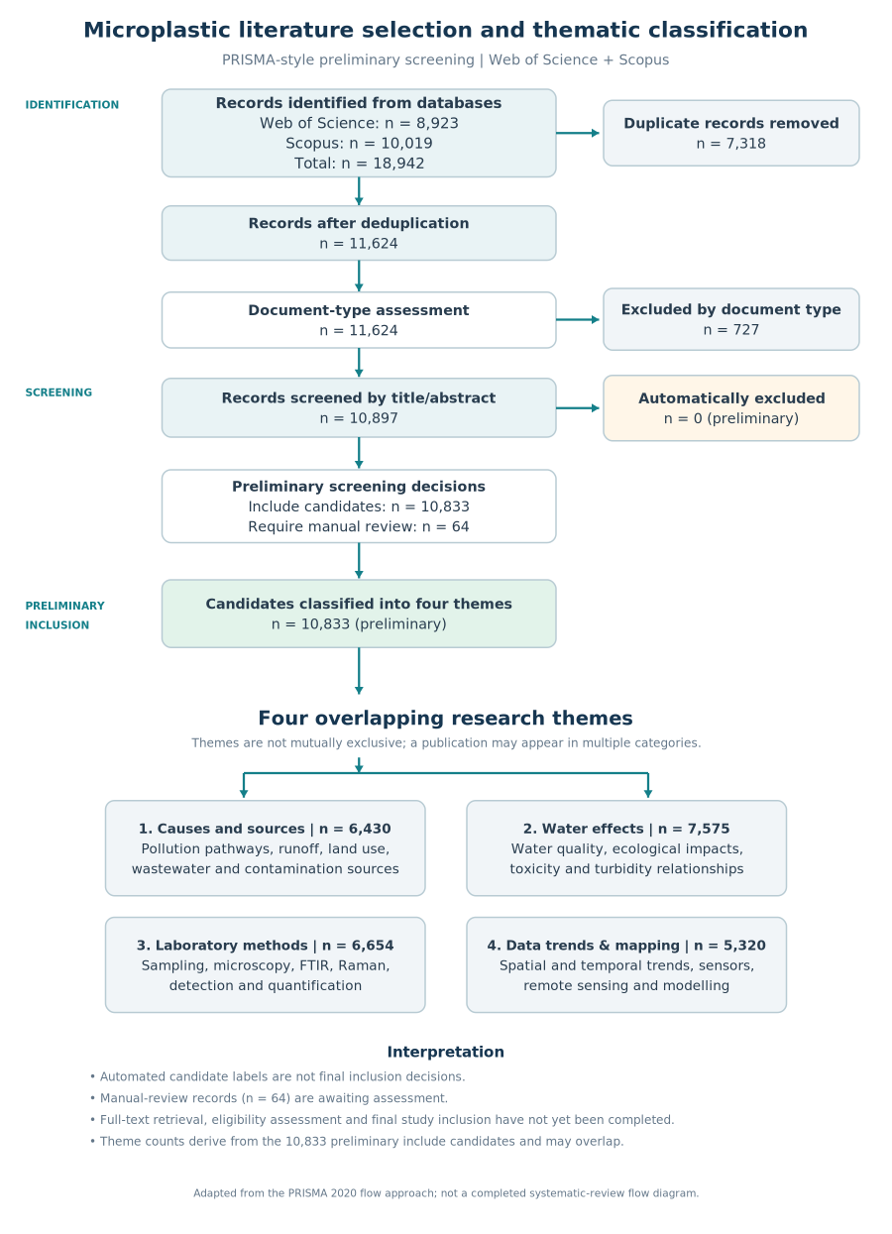
\includegraphics[width=0.70\linewidth,height=.58\textheight,keepaspectratio]{Figures/prisma.png}
\caption{Preliminary PRISMA-style screening and thematic classification; final eligibility and full-text review remain outstanding.}
\end{figure}
\begin{table}[H]\centering\small
\caption{Top-level thematic classifications from 10,833 preliminary include candidates.}
\begin{tabular}{lrr}\toprule
Theme & Papers tagged & Share of candidates \\\midrule
Causes and sources & 6,430 & 59.4\% \\
Water effects & 7,575 & 69.9\% \\
Laboratory methods & 6,654 & 61.4\% \\
Data trends and mapping & 5,320 & 49.1\% \\\bottomrule
\end{tabular}
\end{table}
\begin{figure}[H]
\centering
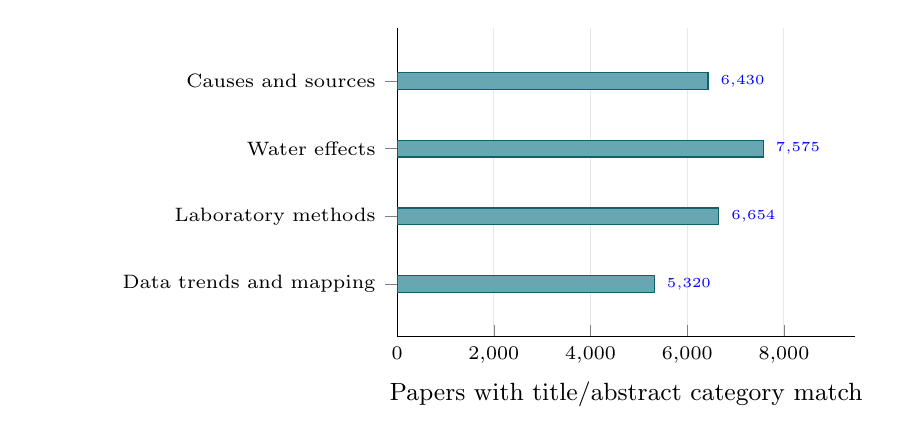
\begin{tikzpicture}
\begin{axis}[
 xbar, bar width=6pt, width=0.61\textwidth, height=5.5cm,
 xmin=0, xmax=9468,
 ymin=-0.65,ymax=3.65,
 ytick={0,1,2,3},
 yticklabels={Data trends and mapping,Laboratory methods,Water effects,Causes and sources},
 yticklabel style={font=\scriptsize,align=right,text width=4.3cm},
 tick label style={font=\scriptsize},
 xlabel={Papers with title/abstract category match},
 xlabel style={font=\small},
 axis x line*=bottom, axis y line*=left,
 xmajorgrids=true, grid style={gray!18},
 nodes near coords, point meta=x,
 every node near coord/.append style={font=\tiny,anchor=west,xshift=1pt},
 enlarge y limits=0.03,
]
\addplot+[draw=teal!80!black,fill=teal!65] coordinates {(5320,0) (6654,1) (7575,2) (6430,3)};
\end{axis}
\end{tikzpicture}
\caption{Four main research themes: automated, overlapping title/abstract subcategory mentions; not verified study findings.}
\end{figure}
\noindent\textbf{Classification note.} The Water Effects keywords reproduce the previously reported twelve-theme classification. The other three themes are newly subdivided using explicit keyword dictionaries supplied in the companion Python file. All four groups are multi-label, and both keyword omissions and false matches are possible. Percentages below use the number of candidates \emph{within that parent theme}, not the overall 10,833 records.
\clearpage
\section{Causes and sources of microplastics}
The largest exploratory source tags concern plastic litter/degradation and wastewater. These labels indicate language in the papers, not source-apportionment results. To identify genuine inputs, quantitative source tracking, site characteristics, and reference sampling are needed.
\begin{figure}[H]
\centering
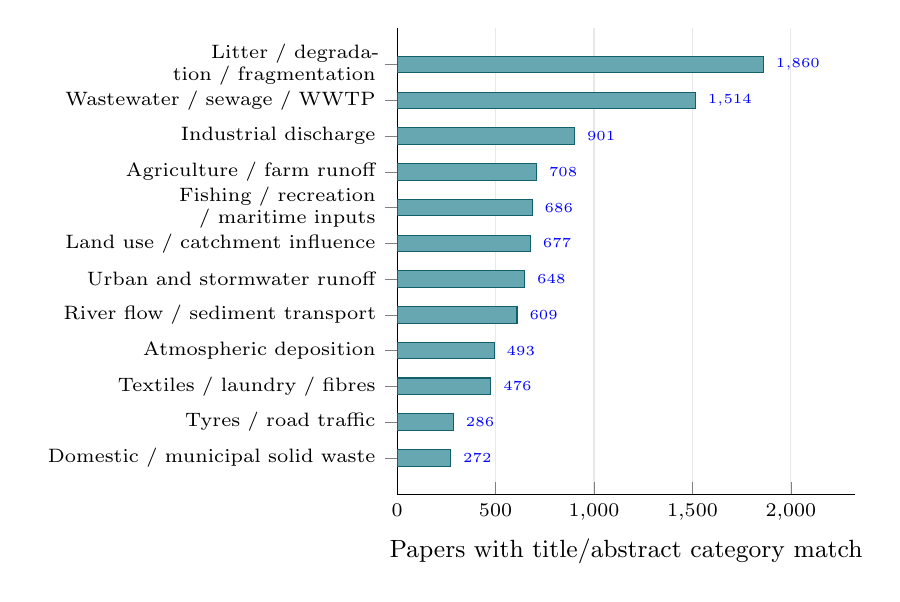
\begin{tikzpicture}
\begin{axis}[
 xbar, bar width=6pt, width=0.61\textwidth, height=7.5cm,
 xmin=0, xmax=2325,
 ymin=-0.65,ymax=11.65,
 ytick={0,1,2,3,4,5,6,7,8,9,10,11},
 yticklabels={Domestic / municipal solid waste,Tyres / road traffic,Textiles / laundry / fibres,Atmospheric deposition,River flow / sediment transport,Urban and stormwater runoff,Land use / catchment influence,Fishing / recreation / maritime inputs,Agriculture / farm runoff,Industrial discharge,Wastewater / sewage / WWTP,Litter / degradation / fragmentation},
 yticklabel style={font=\scriptsize,align=right,text width=4.3cm},
 tick label style={font=\scriptsize},
 xlabel={Papers with title/abstract category match},
 xlabel style={font=\small},
 axis x line*=bottom, axis y line*=left,
 xmajorgrids=true, grid style={gray!18},
 nodes near coords, point meta=x,
 every node near coord/.append style={font=\tiny,anchor=west,xshift=1pt},
 enlarge y limits=0.03,
]
\addplot+[draw=teal!80!black,fill=teal!65] coordinates {(272,0) (286,1) (476,2) (493,3) (609,4) (648,5) (677,6) (686,7) (708,8) (901,9) (1514,10) (1860,11)};
\end{axis}
\end{tikzpicture}
\caption{Causes and sources of microplastics: automated, overlapping title/abstract subcategory mentions; not verified study findings.}
\end{figure}
\begin{table}[H]\centering\footnotesize
\caption{Complete defined subcategory list within causes and sources of microplastics (n=6,430).}
\begin{tabularx}{\linewidth}{@{}Xrr@{}}\toprule Subcategory & Tagged papers & Within-theme share \\ \midrule
Litter / degradation / fragmentation & 1,860 & 28.9\% \\
Wastewater / sewage / WWTP & 1,514 & 23.5\% \\
Industrial discharge & 901 & 14.0\% \\
Agriculture / farm runoff & 708 & 11.0\% \\
Fishing / recreation / maritime inputs & 686 & 10.7\% \\
Land use / catchment influence & 677 & 10.5\% \\
Urban and stormwater runoff & 648 & 10.1\% \\
River flow / sediment transport & 609 & 9.5\% \\
Atmospheric deposition & 493 & 7.7\% \\
Textiles / laundry / fibres & 476 & 7.4\% \\
Tyres / road traffic & 286 & 4.4\% \\
Domestic / municipal solid waste & 272 & 4.2\% \\
\midrule
No defined subcategory term matched & 1,684 & 26.2\% \\
\bottomrule\end{tabularx}\end{table}
\noindent\footnotesize\emph{Counts overlap; a paper can be in several rows. The unmatched count reflects this specific dictionary, not a screening exclusion.}\normalsize
\begin{table}[H]\centering\scriptsize
\caption{Illustrative study-level methodology and reported findings for causes and sources of microplastics. Findings are extracted/paraphrased from supplied abstracts and require full-text verification.}
\begin{tabularx}{\linewidth}{@{}p{2.8cm}XX@{}}\toprule Study & Method or working principle & Abstract-reported observation / implication \\ \midrule
Odora et al. \cite{MPWE00007} & Six Balu River surface-water stations near different industrial operations. & Mean 102.5 $\pm$ 12.83 items/L; site means differed. Observational site differences are not causal source attribution. \\[2pt]
Fan et al. \cite{MPWE00013} & Ten Yangtze River sites; stereomicroscopy and micro-FTIR on water and sediment. & Surface-water abundance 46.7--204 particles/L; separate sediment data. Provides spatial/matrix context. \\[2pt]
Di and Wang \cite{MPWE00126} & Reservoir surface-water and sediment survey with micro-Raman identification. & Water: 1,597--12,611 particles/m$^3$; different patterns were observed in sediments. \\[2pt]
\bottomrule\end{tabularx}\end{table}
\clearpage
\section{Effects on water and aquatic systems}
The twelve established Water Effects labels span physicochemical measurements, biological endpoints, contaminant interactions, and exposure. They overlap and should not be interpreted as numbers of studies confirming adverse effects. For device design, the relevant subset is that reporting paired water-property and laboratory microplastic measurements.
\begin{figure}[H]
\centering
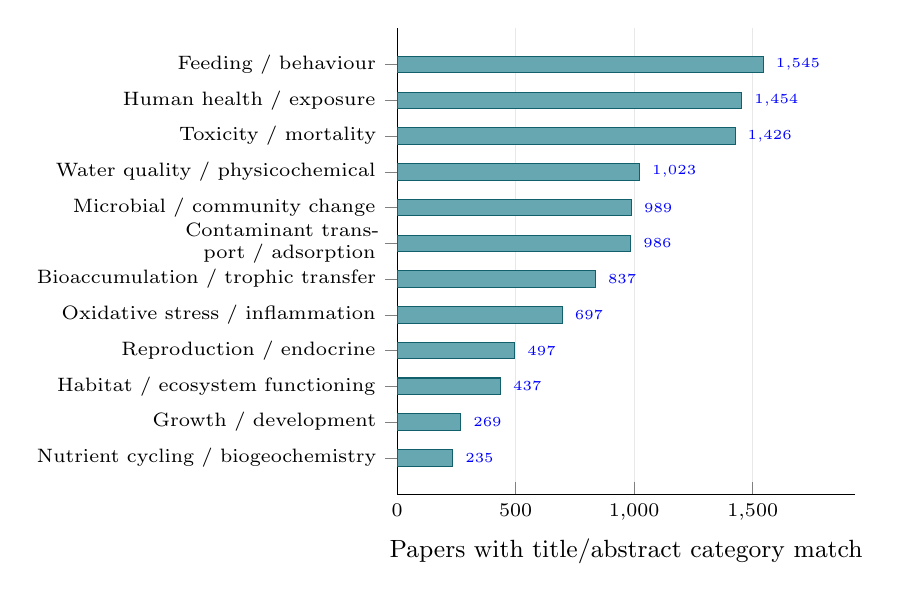
\begin{tikzpicture}
\begin{axis}[
 xbar, bar width=6pt, width=0.61\textwidth, height=7.5cm,
 xmin=0, xmax=1931,
 ymin=-0.65,ymax=11.65,
 ytick={0,1,2,3,4,5,6,7,8,9,10,11},
 yticklabels={Nutrient cycling / biogeochemistry,Growth / development,Habitat / ecosystem functioning,Reproduction / endocrine,Oxidative stress / inflammation,Bioaccumulation / trophic transfer,Contaminant transport / adsorption,Microbial / community change,Water quality / physicochemical,Toxicity / mortality,Human health / exposure,Feeding / behaviour},
 yticklabel style={font=\scriptsize,align=right,text width=4.3cm},
 tick label style={font=\scriptsize},
 xlabel={Papers with title/abstract category match},
 xlabel style={font=\small},
 axis x line*=bottom, axis y line*=left,
 xmajorgrids=true, grid style={gray!18},
 nodes near coords, point meta=x,
 every node near coord/.append style={font=\tiny,anchor=west,xshift=1pt},
 enlarge y limits=0.03,
]
\addplot+[draw=teal!80!black,fill=teal!65] coordinates {(235,0) (269,1) (437,2) (497,3) (697,4) (837,5) (986,6) (989,7) (1023,8) (1426,9) (1454,10) (1545,11)};
\end{axis}
\end{tikzpicture}
\caption{Effects on water and aquatic systems: automated, overlapping title/abstract subcategory mentions; not verified study findings.}
\end{figure}
\begin{table}[H]\centering\footnotesize
\caption{Complete defined subcategory list within effects on water and aquatic systems (n=7,575).}
\begin{tabularx}{\linewidth}{@{}Xrr@{}}\toprule Subcategory & Tagged papers & Within-theme share \\ \midrule
Feeding / behaviour & 1,545 & 20.4\% \\
Human health / exposure & 1,454 & 19.2\% \\
Toxicity / mortality & 1,426 & 18.8\% \\
Water quality / physicochemical & 1,023 & 13.5\% \\
Microbial / community change & 989 & 13.1\% \\
Contaminant transport / adsorption & 986 & 13.0\% \\
Bioaccumulation / trophic transfer & 837 & 11.0\% \\
Oxidative stress / inflammation & 697 & 9.2\% \\
Reproduction / endocrine & 497 & 6.6\% \\
Habitat / ecosystem functioning & 437 & 5.8\% \\
Growth / development & 269 & 3.6\% \\
Nutrient cycling / biogeochemistry & 235 & 3.1\% \\
\midrule
No defined subcategory term matched & 2,346 & 31.0\% \\
\bottomrule\end{tabularx}\end{table}
\noindent\footnotesize\emph{Counts overlap; a paper can be in several rows. The unmatched count reflects this specific dictionary, not a screening exclusion.}\normalsize
\begin{table}[H]\centering\scriptsize
\caption{Illustrative study-level methodology and reported findings for effects on water and aquatic systems. Findings are extracted/paraphrased from supplied abstracts and require full-text verification.}
\begin{tabularx}{\linewidth}{@{}p{2.8cm}XX@{}}\toprule Study & Method or working principle & Abstract-reported observation / implication \\ \midrule
Liu and Li \cite{MPWE00002} & Statistical analysis of microplastics, nitrogen and electrical conductivity in Chinese surface waters. & Electrical conductivity was reported as a mediator (path coefficient 0.521); \emph{not} a validated MP concentration sensor. \\[2pt]
Sau et al. \cite{MPWE02100} & Sampling of 24 urban ponds/lakes with water-quality correlations and SVM classification. & Reported negative associations with turbidity/DO and positive associations with pH and TDS in that dataset; transfer to rivers is untested. \\[2pt]
Rojas-Luna et al. \cite{MPWE00090} & Six lake stations across wet and dry seasons; filtration after digestion and density separation. & Abstract reports mean MP abundance 1.90 particles/L in rainy versus 0.25 particles/L in dry season. \\[2pt]
\bottomrule\end{tabularx}\end{table}
\clearpage
\section{Laboratory and measurement methods}
The method groups describe techniques mentioned in the relevant titles and abstracts. A match does not establish that the technique was actually used in a study. Laboratory reference counting with polymer confirmation and contamination controls is needed to calibrate any proposed field proxy.
\begin{figure}[H]
\centering
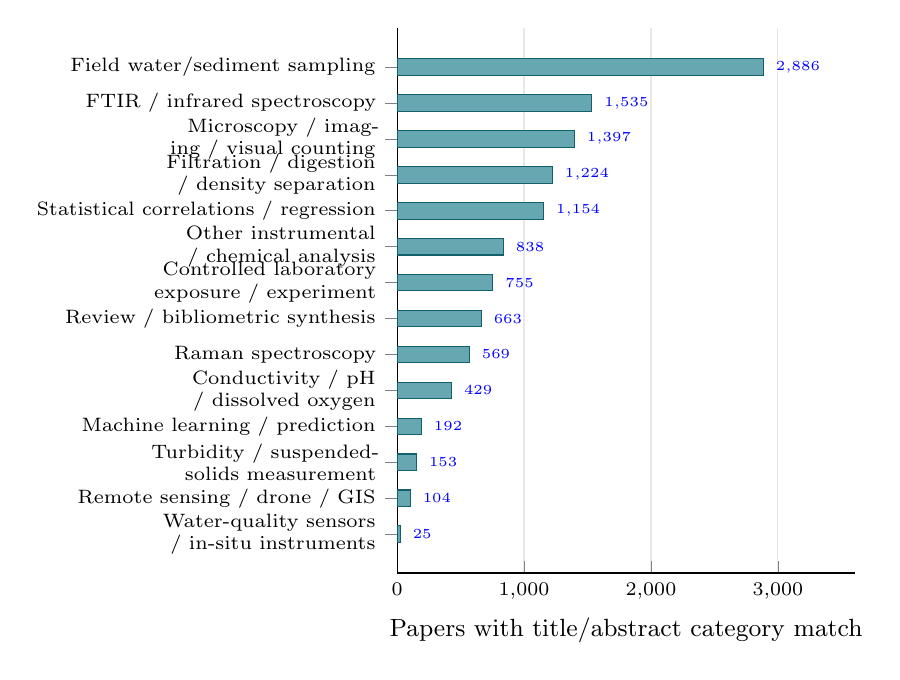
\begin{tikzpicture}
\begin{axis}[
 xbar, bar width=6pt, width=0.61\textwidth, height=8.5cm,
 xmin=0, xmax=3607,
 ymin=-0.65,ymax=13.65,
 ytick={0,1,2,3,4,5,6,7,8,9,10,11,12,13},
 yticklabels={Water-quality sensors / in-situ instruments,Remote sensing / drone / GIS,Turbidity / suspended-solids measurement,Machine learning / prediction,Conductivity / pH / dissolved oxygen,Raman spectroscopy,Review / bibliometric synthesis,Controlled laboratory exposure / experiment,Other instrumental / chemical analysis,Statistical correlations / regression,Filtration / digestion / density separation,Microscopy / imaging / visual counting,FTIR / infrared spectroscopy,Field water/sediment sampling},
 yticklabel style={font=\scriptsize,align=right,text width=4.3cm},
 tick label style={font=\scriptsize},
 xlabel={Papers with title/abstract category match},
 xlabel style={font=\small},
 axis x line*=bottom, axis y line*=left,
 xmajorgrids=true, grid style={gray!18},
 nodes near coords, point meta=x,
 every node near coord/.append style={font=\tiny,anchor=west,xshift=1pt},
 enlarge y limits=0.03,
]
\addplot+[draw=teal!80!black,fill=teal!65] coordinates {(25,0) (104,1) (153,2) (192,3) (429,4) (569,5) (663,6) (755,7) (838,8) (1154,9) (1224,10) (1397,11) (1535,12) (2886,13)};
\end{axis}
\end{tikzpicture}
\caption{Laboratory and measurement methods: automated, overlapping title/abstract subcategory mentions; not verified study findings.}
\end{figure}
\begin{table}[H]\centering\footnotesize
\caption{Complete defined subcategory list within laboratory and measurement methods (n=6,654).}
\begin{tabularx}{\linewidth}{@{}Xrr@{}}\toprule Subcategory & Tagged papers & Within-theme share \\ \midrule
Field water/sediment sampling & 2,886 & 43.4\% \\
FTIR / infrared spectroscopy & 1,535 & 23.1\% \\
Microscopy / imaging / visual counting & 1,397 & 21.0\% \\
Filtration / digestion / density separation & 1,224 & 18.4\% \\
Statistical correlations / regression & 1,154 & 17.3\% \\
Other instrumental / chemical analysis & 838 & 12.6\% \\
Controlled laboratory exposure / experiment & 755 & 11.3\% \\
Review / bibliometric synthesis & 663 & 10.0\% \\
Raman spectroscopy & 569 & 8.6\% \\
Conductivity / pH / dissolved oxygen & 429 & 6.4\% \\
Machine learning / prediction & 192 & 2.9\% \\
Turbidity / suspended-solids measurement & 153 & 2.3\% \\
Remote sensing / drone / GIS & 104 & 1.6\% \\
Water-quality sensors / in-situ instruments & 25 & 0.4\% \\
\midrule
No defined subcategory term matched & 990 & 14.9\% \\
\bottomrule\end{tabularx}\end{table}
\noindent\footnotesize\emph{Counts overlap; a paper can be in several rows. The unmatched count reflects this specific dictionary, not a screening exclusion.}\normalsize
\begin{table}[H]\centering\scriptsize
\caption{Illustrative study-level methodology and reported findings for laboratory and measurement methods. Findings are extracted/paraphrased from supplied abstracts and require full-text verification.}
\begin{tabularx}{\linewidth}{@{}p{2.8cm}XX@{}}\toprule Study & Method or working principle & Abstract-reported observation / implication \\ \midrule
Ermolin \cite{MPWE00061} & Review of water/sediment sampling, size/density separation and digestion methods. & Explains why sample preparation and recovery controls must be selected for the matrix; no single universal approach. \\[2pt]
Rojas-Luna et al. \cite{MPWE00090} & 72 water samples; H$_2$O$_2$ digestion, NaCl density separation, and filtration. & Observed abundance ranged from zero to 3.83 particles/L; laboratory extraction method affects the reportable fraction. \\[2pt]
Fan et al. \cite{MPWE00013} & Digital stereomicroscope for particle counting and micro-FTIR for polymer identification. & Illustrates the distinction between suspected particle enumeration and polymer confirmation. \\[2pt]
Narwal and Katyal \cite{MPWE00012} & Stereomicroscopy, electron microscopy and ATR-FTIR in surface waters. & Abstract reports 16--28 particles/L and polyethylene/polypropylene/polystyrene in analysed samples. \\[2pt]
\bottomrule\end{tabularx}\end{table}
\clearpage
\section{Data trends, monitoring and spatial mapping}
This exploratory categorisation describes spatial, temporal, monitoring, modelling and imaging vocabulary. Studies predicting water attributes from images must be distinguished from studies estimating laboratory-confirmed microplastic concentrations with independent validation.
\begin{figure}[H]
\centering
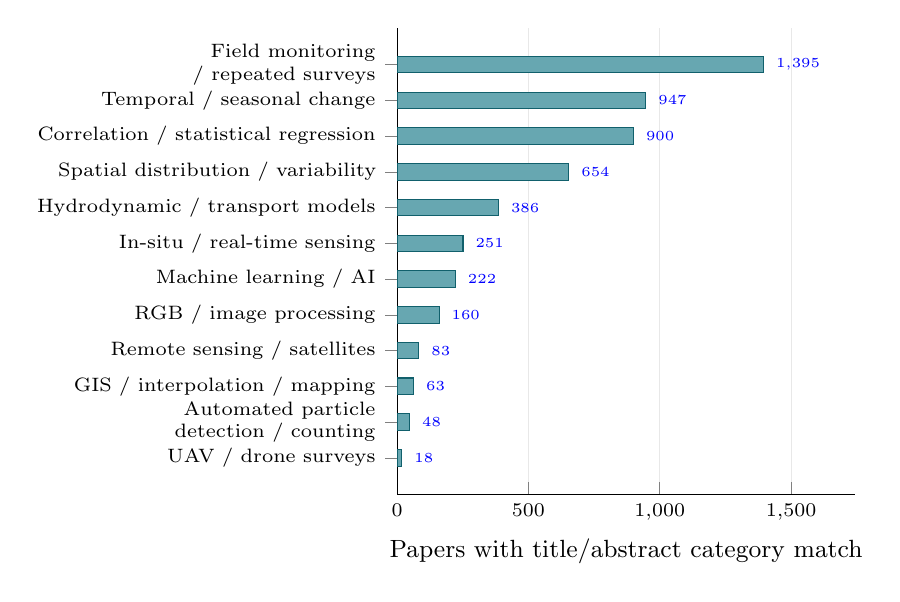
\begin{tikzpicture}
\begin{axis}[
 xbar, bar width=6pt, width=0.61\textwidth, height=7.5cm,
 xmin=0, xmax=1743,
 ymin=-0.65,ymax=11.65,
 ytick={0,1,2,3,4,5,6,7,8,9,10,11},
 yticklabels={UAV / drone surveys,Automated particle detection / counting,GIS / interpolation / mapping,Remote sensing / satellites,RGB / image processing,Machine learning / AI,In-situ / real-time sensing,Hydrodynamic / transport models,Spatial distribution / variability,Correlation / statistical regression,Temporal / seasonal change,Field monitoring / repeated surveys},
 yticklabel style={font=\scriptsize,align=right,text width=4.3cm},
 tick label style={font=\scriptsize},
 xlabel={Papers with title/abstract category match},
 xlabel style={font=\small},
 axis x line*=bottom, axis y line*=left,
 xmajorgrids=true, grid style={gray!18},
 nodes near coords, point meta=x,
 every node near coord/.append style={font=\tiny,anchor=west,xshift=1pt},
 enlarge y limits=0.03,
]
\addplot+[draw=teal!80!black,fill=teal!65] coordinates {(18,0) (48,1) (63,2) (83,3) (160,4) (222,5) (251,6) (386,7) (654,8) (900,9) (947,10) (1395,11)};
\end{axis}
\end{tikzpicture}
\caption{Data trends, monitoring and spatial mapping: automated, overlapping title/abstract subcategory mentions; not verified study findings.}
\end{figure}
\begin{table}[H]\centering\footnotesize
\caption{Complete defined subcategory list within data trends, monitoring and spatial mapping (n=5,320).}
\begin{tabularx}{\linewidth}{@{}Xrr@{}}\toprule Subcategory & Tagged papers & Within-theme share \\ \midrule
Field monitoring / repeated surveys & 1,395 & 26.2\% \\
Temporal / seasonal change & 947 & 17.8\% \\
Correlation / statistical regression & 900 & 16.9\% \\
Spatial distribution / variability & 654 & 12.3\% \\
Hydrodynamic / transport models & 386 & 7.3\% \\
In-situ / real-time sensing & 251 & 4.7\% \\
Machine learning / AI & 222 & 4.2\% \\
RGB / image processing & 160 & 3.0\% \\
Remote sensing / satellites & 83 & 1.6\% \\
GIS / interpolation / mapping & 63 & 1.2\% \\
Automated particle detection / counting & 48 & 0.9\% \\
UAV / drone surveys & 18 & 0.3\% \\
\midrule
No defined subcategory term matched & 2,030 & 38.2\% \\
\bottomrule\end{tabularx}\end{table}
\noindent\footnotesize\emph{Counts overlap; a paper can be in several rows. The unmatched count reflects this specific dictionary, not a screening exclusion.}\normalsize
\begin{table}[H]\centering\scriptsize
\caption{Illustrative study-level methodology and reported findings for data trends, monitoring and spatial mapping. Findings are extracted/paraphrased from supplied abstracts and require full-text verification.}
\begin{tabularx}{\linewidth}{@{}p{2.8cm}XX@{}}\toprule Study & Method or working principle & Abstract-reported observation / implication \\ \midrule
Sau et al. \cite{MPWE02100} & Sentinel-2 remote sensing, GIS and support-vector-machine analysis. & Study reports morphology SVM accuracy of 89\%; remote-sensing validation values are study-specific and require independent replication. \\[2pt]
Chabot and Marteinson \cite{MPWE04211} & Review of aerial spectral, surface-roughness and indirect-proxy approaches. & Identifies approaches as largely experimental rather than established operational MP measurements. \\[2pt]
Liu et al. \cite{MPWE01416} & Polarised scattering at 120$^\circ$ and machine-learning classification. & Experimental discrimination of polystyrene particles from algae/natural samples; not yet a calibrated river-wide concentration map. \\[2pt]
Rojas-Luna et al. \cite{MPWE00090} & Repeated wet/dry season field sampling. & Seasonal difference illustrates why spatial maps need sampling date, rainfall and measurement uncertainty. \\[2pt]
\bottomrule\end{tabularx}\end{table}
\clearpage
\section{Compiled method--effect comparison and next decisions}
\begin{table}[H]\centering\footnotesize
\caption{Connecting literature methods and effects to the proposed controlled-sample experiment.}
\begin{tabularx}{\linewidth}{@{}p{3.0cm}XX@{}}\toprule
Observed / studied relationship & Example literature evidence & What to validate in our chemistry laboratory \\ \midrule
Spatial differences in particle abundance & Balu and Yangtze sampling \cite{MPWE00007,MPWE00013} & Replicate reference concentration by site and time; retain sample volume and GPS position. \\
MPs and nitrogen / conductivity & Surface-water statistical analysis \cite{MPWE00002} & Ionic strength and turbidity must vary independently of MP dose; assess whether adding MP improves prediction. \\
Wet/dry season variation & Repeated seasonal lake sampling \cite{MPWE00090} & Test model transfer across time and rainfall conditions. \\
Particle recovery and chemical identification & Sample-preparation review and stereomicroscope--FTIR surveys \cite{MPWE00061,MPWE00013,MPWE00012} & Quantify blank contamination, spike recovery, repeatability and polymer-confirmation rate. \\
Optical scattering and particle discrimination & Polarised-scattering experiments \cite{MPWE01416} & Challenge the sensor with algae, mineral sediments, differently sized polymers and mixed matrices. \\
Spatial prediction and aerial imagery & GIS/SVM study and aerial review \cite{MPWE02100,MPWE04211} & Train with georeferenced paired sensor--reference data; validate on completely withheld sites and days. \\
\bottomrule\end{tabularx}
\end{table}
\begin{figure}[H]\centering
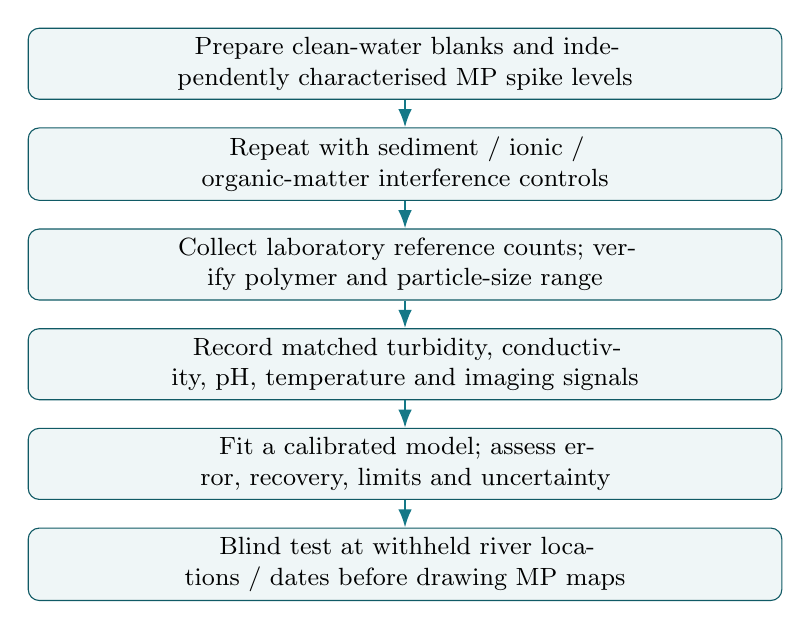
\begin{tikzpicture}[node distance=3.5mm,b/.style={draw=teal!75!black,rounded corners,fill=teal!7,align=center,text width=0.77\linewidth,minimum height=8mm,font=\small},>=Latex]
\node[b](standards){Prepare clean-water blanks and independently characterised MP spike levels};
\node[b,below=of standards](matrices){Repeat with sediment / ionic / organic-matter interference controls};
\node[b,below=of matrices](reference){Collect laboratory reference counts; verify polymer and particle-size range};
\node[b,below=of reference](proxy){Record matched turbidity, conductivity, pH, temperature and imaging signals};
\node[b,below=of proxy](model){Fit a calibrated model; assess error, recovery, limits and uncertainty};
\node[b,below=of model](field){Blind test at withheld river locations / dates before drawing MP maps};
\foreach \x/\y in {standards/matrices,matrices/reference,reference/proxy,proxy/model,model/field} \draw[->,thick,teal](\x)--(\y);
\end{tikzpicture}
\caption{Proposed laboratory-to-field validation chain. This is a project plan, not a tested result.}
\end{figure}
\section{Interpretation and limitations}
The four top-level counts originate from preliminary screening, not final inclusion; 64 additional records await manual review. Subcategory labels are automated mentions in title/abstract text. Their counts may include reviews, descriptions of prior methods or hypotheses, and do not determine effectiveness, causality or evidence quality. The study examples illustrate different working principles but do not represent a quantitative synthesis of all candidate papers. Before final thesis conclusions, complete full-text screening, confirm reported effects and citations, and pre-specify the calibration and external-validation protocol with the chemistry laboratory.
\printbibliography[title={References}]
\end{document}
